\documentclass[12pt]{article}
\usepackage{graphicx}
\usepackage{amsmath}
\graphicspath{ {./images/} }
\title{Ch 226 HW 3}
\author{Patryk Kozlowski}
\date{\today}
\begin{document}
\maketitle
\section{}
Qmix calculates phase matching conditions for a specified crystal and wavelengths. Use Qmix to calculate the crystal orientation $\theta$ you would need for SHG with an 800 nm pump in a BBO crystal. What value of $d_{eff}$ do you get?
\subsection{Answer}
This is the output we got when we click run with these settings on Qmix:
\begin{figure}
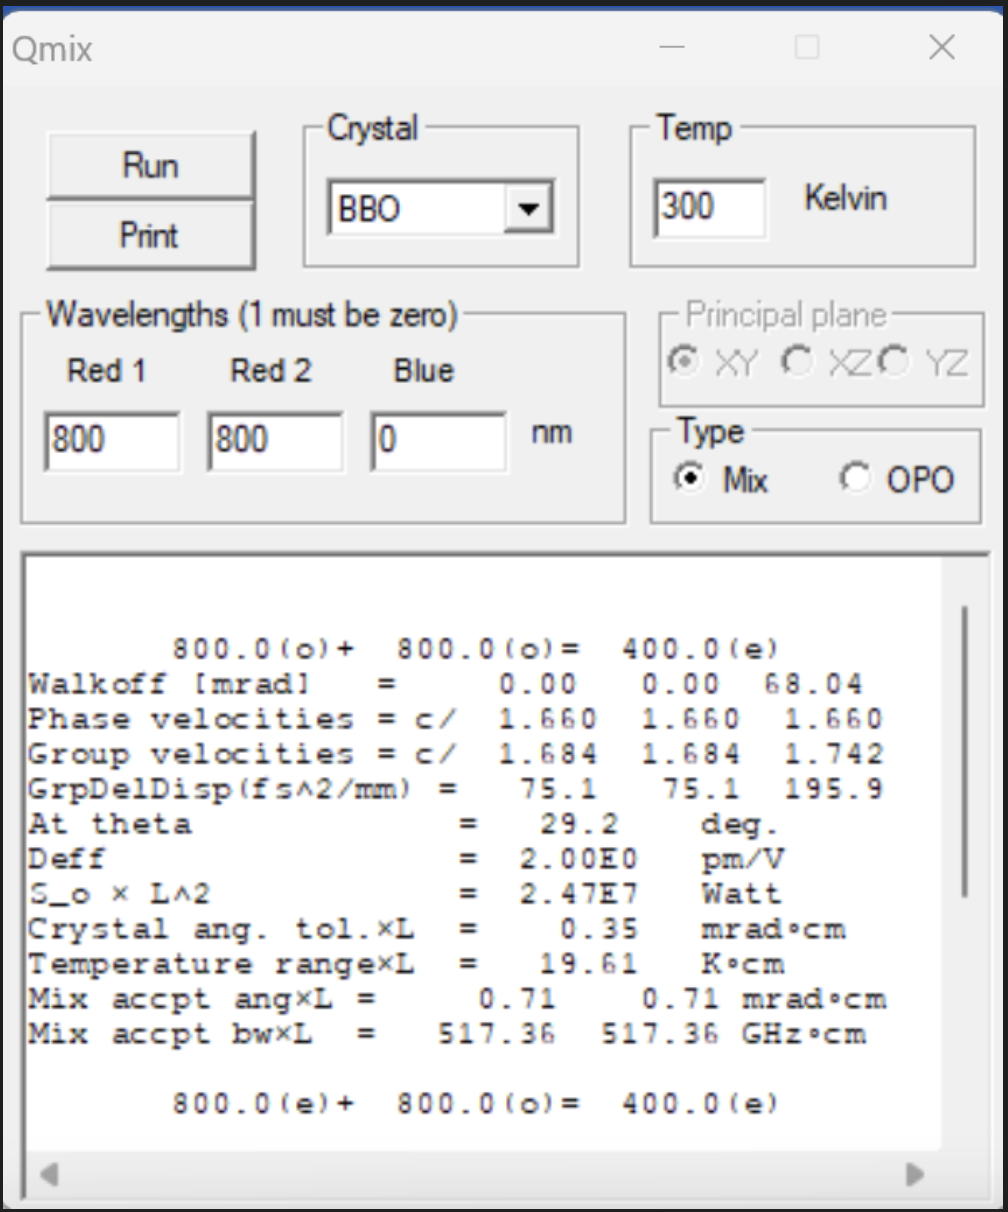
\includegraphics[width=\textwidth]{1.png}
\end{figure}
Some useful features to note are that we have 2 input beams, both with a wavelength of 800 nanometers and these combine to a beam with a wavelength of 400 nanometers. It should also be noted that the input beams are along the ordinary axis while the output beam is along the extraordinary. The crystal orientation $\theta$ is 29.2 degrees and the value of $d_{eff}$ is 2 pm/V.
\newpage
\section{}
An optical parametric oscillator has a 355 nm pump laser with a pulse duration of 7 ns. You want to do type I mixing in an OPO to access a frequency range of 400 - 2600 nm, use the opoangles calculation to determine which of the following crystals would be best suited for this energy range. Explain why you chose that crystal and why the others would not work as well.
\begin{itemize}
\item DKDP
\item KNbO3
\item KTP\_F
\item LBO
\end{itemize}
\subsection{Answer}
We used the reciprocal angle calculation to determine the best crystal for this energy range. The output for the 4 chosen crystals is shown below:
\newpage
\begin{figure}
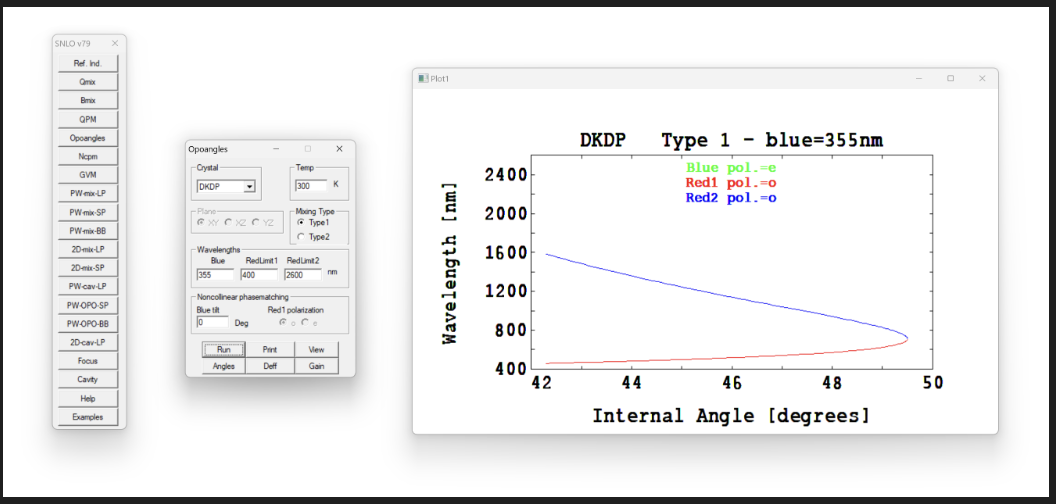
\includegraphics[width=\textwidth]{2.png}
\end{figure}
\begin{figure}
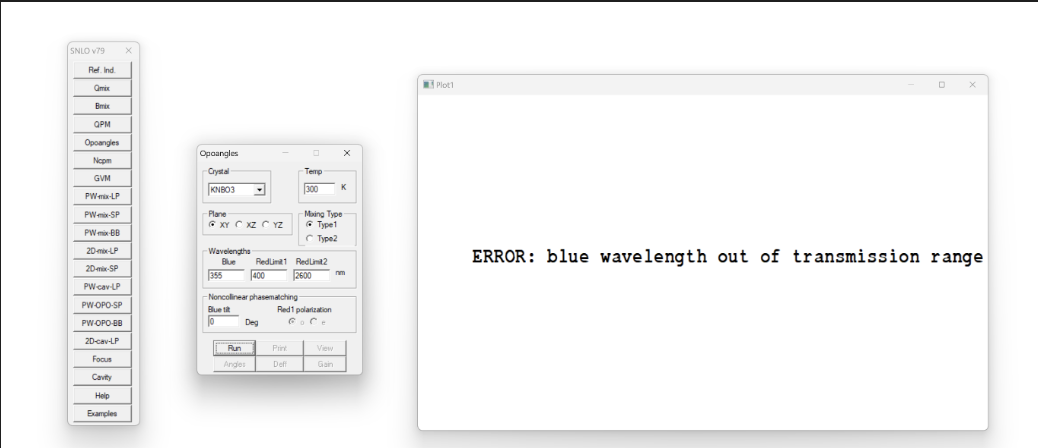
\includegraphics[width=\textwidth]{3.png}
\end{figure}
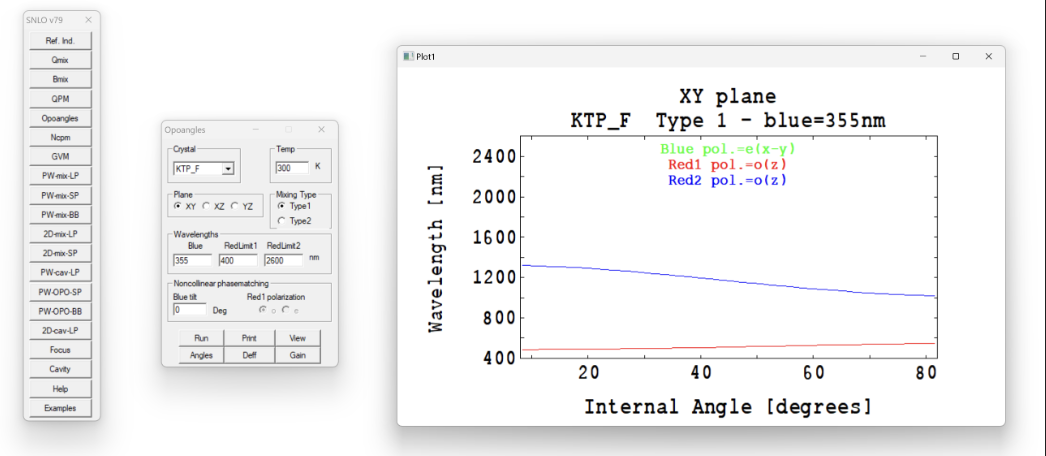
\includegraphics[width=\textwidth]{4.png}
\begin{figure}
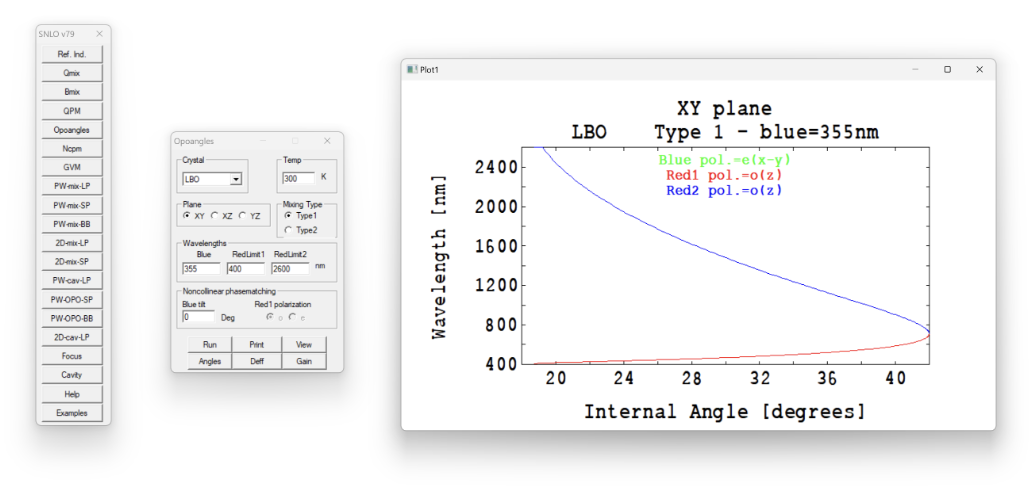
\includegraphics[width=\textwidth]{5.png}
\end{figure}

The blue wavelength corresponds to our pump pulse, the red limits correspond to the frequency range that we want to access. The plots can be interpreted as follows: on the horizontal axis is the internal angle which we are free to change arbitrarily by rotation of the crystal. What we really want to do is to choose an internal angle for a given crystal that gives access to the widest range of frequencies, namely we want the red and blue curves to be closest to 400 nanometers and 2400 nanometers, respectively. Given this information, the crystal that best is able to encompass this desired frequency range is LBO as it covers the desired frequency range at an internal angle of 20 degrees. Also note that the pump pulse wavelength was not at all compatible with KNbO3, and so when we tried to run it in the program, an error occurred.



\end{document}
